\documentclass{article}

% Language setting
% Replace `english' with e.g. `spanish' to change the document language
\usepackage[english]{babel}

% Set page size and margins
% Replace `letterpaper' with `a4paper' for UK/EU standard size
\usepackage[letterpaper,top=2cm,bottom=2cm,left=3cm,right=3cm,marginparwidth=1.75cm]{geometry}

% Useful packages
\usepackage{amsfonts}
\usepackage{amsmath}
\usepackage{graphicx}
\usepackage[utf8]{inputenc}
\usepackage[colorlinks=true, allcolors=blue]{hyperref}

\title{MTH2021 Computed Tomography Report}
\author{Maeve McSherry 40394838}

\begin{document}
\maketitle


\section{Introduction}

What is Computed Tomography? (CT scan/CAT scan)

Computed Tomography is a medical imaging technique that combines a series of X-ray images taken from different angles that are analysed mathematically to create cross-sectional (2D) or 3D images of the inside of a patient's body. This is known as mathematical reconstruction. This technique is non-invasive and painless. 

How was Computer Assisted Tomography developed?

An electrical engineer called Godfrey Hounsfield had an idea to examine and view organs from outside the body. Hounsfield's idea was centered on the fact that the intensity of an X-ray beam is reduced when it passes through an object, a process called attenuation. To observe the different attenuation patterns from a human object by directing an X-ray beam through it from different angles, we could distinguish between different types of tissues and reconstruct an image of a 'slice' of that object. However, South African physicist Allan Cormack had already shown in theory that such an image could be obtained, but he did not create an instrument that could carry this out. Hounsfield began to turn his idea into a working product. As a result, Godfrey Hounsfield and Allan Cormack were both awarded the Nobel Prize in Physiology or Medicine 1979 for "the development of computed assisted tomography". \cite{nobelprize_ct}

Why is Computed Tomography important?

It allows physicians to identify health complications such as tumors, infections and injuries and diagnose patients effectively.

In this report we will look at the mathematical principles behind computed tomography image reconstruction.


\section{Mathematical Background}

\subsection{The Radon Transform}

Computed Tomography reconstructs an image by combining measurements from different directions using a computational algorithm. Looking at this mathematically, we consider a two-dimensional object represented by a function $u(x,y)$, which we assume lies within a unit circle.

A CT scanner measures how much radiation passes through the object along straight lines. A flat detector is placed along the tangent of the unit circle. This detector takes measurements at different angles around the object, for a given angle $\theta$. Any point/position along the detector line $l(t, \theta)$ can be described by a displacement parameter $t$ $\in$ $\mathbb{R}$, how far the line is from the origin. We can therefore calculate each measurement, for the function $A(t, \theta)$: \cite{Chapter8_ct}
\[A(t, \theta) = \int_{l(t,\theta)} u(x,y) ds \]

A collection of these measurements reconstruct the original image. This collection of projections is called the Radon Transform.

\subsection{The Fourier Slice Theorem} \label{sec:fourier_slice}

We need to reconstruct the function $u(x,y)$ from the collection of images $A(t, \theta)$. 

The Fourier slice theorem states that the 1D Fourier transform of a projection is equivalent to a slice through the 2D fourier transform of the image at the same angle as the projection \cite{fourierslice}. The Fourier transform theory begins with the 1D continuous transform, defined as follows:
\[\hat{A}(k, \theta) = \int_{-\infty}^{\infty} A(t, \theta) e^{-2\pi ikt}dt\]
Where $e^{-2\pi ikt}$ is a complex exponential and k is the frequency variable. This converts the projection into frequency space.

Next, we carry out coordinate transformation as this lets us build a 2D fourier plane. Let $\hat{u}(k_{x}, k_{y})$ be the 2D Fourier transform of the original image $u(x,y)$. 
\[\hat{u}(k_{x}, k_{y}) = \int \int^{\infty}_{-\infty} u(x,y) e^{-2\pi i(k_{x}x + k_{y}y)}dxdy = \int \int^{\infty}_{-\infty} u(x,y) e^{-2\pi i(kcos\theta x + ksin\theta y)}dxdy \]
Then
\[\hat{A}(k, \theta) = \hat{u}(k_{x}, k_{y}) = \hat{u}(kcos\theta , ksin\theta)\]
with 
\[k_{x} = kcos\theta, k_{y} = ksin\theta, k = \sqrt{k_{x}^{2} + k_{y}^{2}}\]

\cite{Ft_pt2}. This result shows that the 1D Fourier transform taken at an angle $\theta$ is equivalent to the values of the 2D Fourier transform of the object along a line at the same angle. 

Why this allows image reconstruction?

We can obtain multiple slices of the Fourier transform of the object by collecting projections at different angles, and these projections fill the frequency plane which allows for the original image $u(x,y)$ to be reconstructed by the Inverse Radon Transform.


\subsection{Inverse Radon Transform: Fourier Reconstruction}

As stated in section \ref{sec:fourier_slice} the Fourier slice theorem establishes that the 1D Fourier transform of a projection corresponds to a slice through the 2D fourier transform of the image at the same angle $\theta$ as the projection. In order for these to be equivalent, coordinate transformation needs to take place. More specifically, the coordinate system must be rotated to match the angle $\theta$ of the projection, put all values of the 1D function $\hat{A}(k,\theta)$ on a polar grid to obtain the 2D function $\hat{u}(k_{x}, k_{y})$. Fourier data must be expressed in Cartesian frequency coordinates to obtain $\hat{u}(k_{x},k_{y})$.
Convert 
\[(k, \theta)\]
to Cartesian coordinates $(k_{x}, k_{y})$ for
\[k_{x} = kcos\theta\]
\[k_{y} = ksin\theta\]
This allows us to build a 2D Fourier plane. \cite{Ft_pt2}

Once we fill the fourier plane, how do we recover the image? 

The recovery process of the orginal image $u(x,y)$, given the Radon transform $A(t,\theta)$, is called the inverse Radon transform. We can use the Inverse Fourier Transform to mathematically reconstruct the image $u(x,y)$. The formula is as follows: 
\[u(x,y) = \int \int \hat{u}(k_x, k_y) e^{2\pi i(k_{x}x + k_{y}y)}dk_{x}dk_{y}\]
The sign on the functions' exponent is changed from $-1$ to $1$. The equation we have works with cartesian coordinates $(k_x , k_y)$. However, we need to rewrite the equation in polar frequency coordinates $(k, \theta)$, not cartesian $(k_x , k_y)$ as this is what the Fourier data from the projections are expressed in. This is where Filtered Back-Projection comes into place. \cite{Back_projection}

\subsection{Filtered Back-Projection}

Using the coordinate transformation 
\[k_x = kcos\theta\]
\[k_y = ksin\theta\]
The area element changes from
\[dk_x dk_y = |k|dkd\theta\]
Therefore, we take the polar version of the inverse Fourier transform to be: 
\[u(x,y) = \int^{\pi}_{0} \int^{\infty}_{-\infty} |k| \hat{A}(k,\theta)e^{ik(xcos\theta + ysin\theta)}dkd\theta\]
Why do we multiply by the absolute value of $k$?

The $|k|$ is the Jacobian determinant that is introduced when converting from cartesian to polar coordinates. It acts as a frequency filter. Simple back-projection by itself creates a blurry image due to too many low frequencies being projected back. To improve the image, we can introduce weights that counter-act this imbalance in favour of the high frequencies. This is where we introduce $|k|$ which is known as a Ramp filter which acts as a high pass filter, reducing low frequencies and increasing high frequencies. This sharpens and enhances the image. 

After filtering, the projections are transformed back into spatial space. The filtered projections are integrated back across the image along the same lines that were originally measured. From the inverse Fourier formula we see that the exponential term 
\[e^{ik(xcos\theta + ysin\theta)}\]
which arises after coordinate transformation corresponds to this. It represents a plane wave contribution at each point $(x,y)$. Adding all the contributions from all frequencies and angles reconstructs the image. \cite{Chapter8_ct}

Let us consider the Fourier coefficient at $k=0$. This is the zero frequency component which represents the average intensity of the image. 

As we know, in the reconstruction formula used for CT imaging, the Fourier coefficients are multiplied by a weighting factor $|k|$. At $k=0$, this weight becomes
\[|k| = 0\]
When multiplied, this removes the constant background intensity from the reconstruction. This does not affect the visibility of the structures in an image. Clinicians are interested in changes in attenuation in CT images, which is not impacted by this factor.


\subsection{Numerical Implementation and FFT Considerations}

We must look at coding and numerical issues that arise in Computed Tomography. Let us take a look at FFT interval issues.

 The Discrete Fourier Transform (DFT) is a mathematical function and the Fast Fourier Transform (FFT) is an algorithm for computing that function, it decomposes it into sine and cosine components at different frequencies \cite{fft2021}. Python's NumPy routine \texttt{np.fft} computes the Discrete Fourier Transform over the interval $[0, 2L]$ while the desired Fourier series uses $[-L, L]$. When the Fourier transform is needed on an interval $[-L, L]$, this difference in intervals requires the Fourier coefficients obtained from \texttt{np.fft} to be adjusted before they can be used in the reconstruction.

 A change in variables can map the interval $[-L, L]$ to $[0,2L]$. If we denote $t'$ as the coordinate used by the FFT routine, we can substitute this for
 \[t' = t + L\]
 The complex Fourier coefficient for interval $[-L, L]$ can be written as 
 \[A_k = 1/2L \int^{L}_{-L} A(t)e^{-ikt}dt\]
Substituting $t'=t+L$, this becomes an integral over the interval $[0, 2L]$ which changes the exponential term to
\[e^{-ikL}\]
Therefore, in order to obtain the Fourier coefficients for $[-L, L]$, the coefficients returned by the FFT must be multiplied by a complex phase factor 
\[e^{ikL}\]
which has a unit magnitude
\[|e^{ikL}| = 1\]
Why should the magnitude of each Fourier coefficient stay the same?

Multiplying the Fourier coefficients by the complex phase factor $e^{ikL}$ changes only their phase, not their magnitude. So the overall magnitude of each coefficient remains unchanged. \cite{fft2021} \cite{fft1997}

\section{Computational Part of Tomography}

\subsection{Computational Method}

This section describes how the reconstruction was implemented. 

The reconstruction is implemented in Python using numerical libraries such as NumPy. The projection data $A(t, \theta)$ is first transformed into the frequency domain using the Fast Fourier Transform (FFT) implemented through \texttt{np.fft}. This computes the discrete Fourier transform of the projection. The resulting Fourier coefficients are then adjusted due to the interval $[0, 2L]$ used by the FFT routine and mapped to their corresponding wave numbers using \texttt{np.fft.fftfreq}. The weighting factor $|k|$ is applied to the Fourier coefficients to create the filtering step required for Filtered Back-Projection. After filtering, the projection data is transformed back into spatial space and back-projected across the image domain. Contributions from all angles are then summed to obtain the reconstructed image. We can see this is in  figure \ref{fig:Recon}.

\subsection{Results}
\begin{figure}[!htbp]
    \centering
    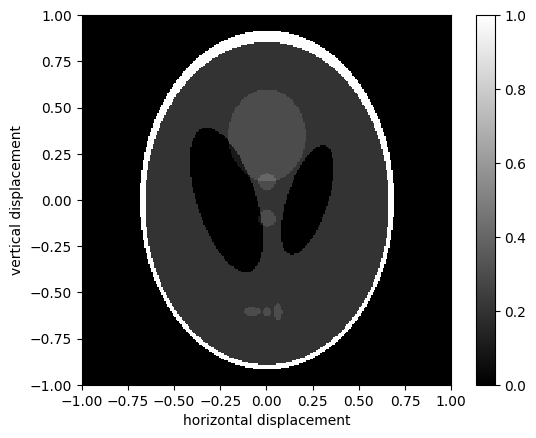
\includegraphics[width=0.5\linewidth]{shepplogan.png}
    \caption{\label{fig:ShL}This is the Shepp-Logan phantom image. The function to make this starting image is called \texttt{sheplog}.}
\end{figure}

\begin{figure}
    \centering
    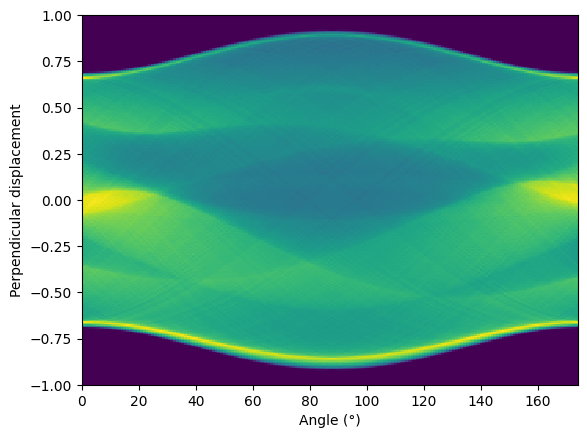
\includegraphics[width=0.5\linewidth]{Radontrans.png}
    \caption{\label{fig:RT}This is the resulting image when the Radon Transform is applied to the Shepp-Logan Phantom.}
\end{figure}

\begin{figure}
    \centering
    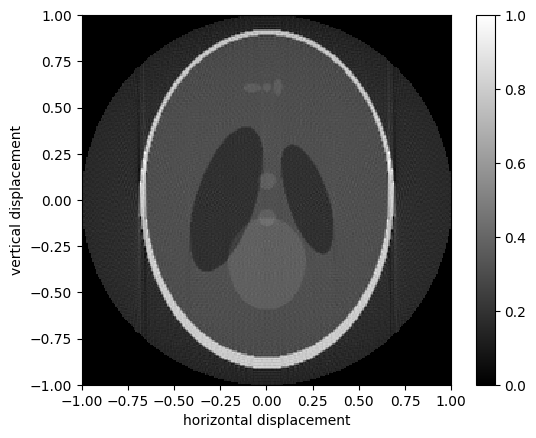
\includegraphics[width=0.5\linewidth]{reconstructed.png}
    \caption{\label{fig:Recon} This is the final reconstructed 2D image obtained using Filtered Back-Projection. The application of the $|k|$ filter improved the sharpness of the edges. Without this filtering step, the reconstructed image appeared blurry due to the accumulation of low frequency components. This final image demonstrates that the algorithm successfully recovered the major structural features of the original Shepp-Logan phantom image.}
\end{figure}

\newpage
We can see that there are some discrepancies between the reconstructed image and the original image. For example, there are faint vertical streaks due to a limited number of projection angles. These small artifacts are expected from numerical approximations in the reconstruction.

\section{Conclusion}
In this report, we investigate the mathematical principles involved with computed tomography. The theory was introduced through the concept of line integrals and the Radon transform, followed by the Fourier Slice Theorem and inverse Radon Transform in order to reconstruct the image. The computational implementation demonstrated how projection data can be reconstructed numerically using Fourier methods and the Fast Fourier Transform. These results illustrate how the mathematical theory and computational techniques are combined in CT reconstruction, and their practical importance in modern medical imaging.

\bibliographystyle{alpha}
\bibliography{References}

\end{document}
